%!TEX root = ../thesis.tex

\section{Family of graphs not $\mathbf{k}$-sided for any $\mathbf{k}$}
\thispagestyle{plain}
  \label{s:fix}
  In this section we will show the following theorem.

  \begin{thrm}
    \label{fix:th:family}
      There is a family of graphs $G_k$ that for any $k \in \N$ has members that are not $k$-sided.
  \end{thrm}

  All members of this family contain separating $4$-cycles.
  If there is no $k$-sided rectangular dual for a certain corner assignment $\ext G_k$ of $G_k$. There may still be another corner assignment of $G_k$ admitting a $k$-sided dual.
  However, if we view $\ext G_k = H_k$ as a graph in its own right, then $G_k$ is the interior of a separating $4$-cycle of $H_k$ and we will show in Lemma \ref{lm:fix:fourCycleInteriorColor} this implies that $G_k$ (as induced subgraph) has to be colored in accordance with the corner assignment $\ext G_k$. Hence we first have to proof some lemma's before we can turn to the proof of Theorem \ref{fix:th:family}.

  \begin{lemma}
    \label{lm:interiorRectangle}
    Let $\C$ be a separating $4$-cycle of a corner assignment $\ext G$ with interior $I$. Then in any rectangular dual of $\ext G$ the region enclosed by the rectangles dual to the vertices in $\C$ is a rectangle.
  \end{lemma}
  \begin{proof}
    The interior $I$ of $\C$ will be represented by some rectilinear shape in every rectangular dual $\L$ of G. Such a shape must have at least $4$ clockwise right turns if we travel its boundary in a clockwise direction otherwise the shape is not closed.

    On the other hand such a clockwise turn can not occur due to a single rectangle. Instead such a turn can only occur when two rectangles are adjacent to each other. Since a $4$-cyle represents only $4$ pairs of adjacent rectangles the representation of $I$ in $\L$ can only have $4$ clockwise turns. Hence it must be a rectangle, the only rectilinear shape with just $4$ clockwise turns
  \end{proof}

  \begin{lemma}
  \label{lm:fix:fourCycleInteriorColor}
  Let $\C$ be a separating $4$-cycle of $\ext G$ with interior $I$. We can label the vertices $a$, $b$, $c$ and $d$ in clockwise order around $I$ such that all interior edges incident to $a, b, c$ and $d$ are incoming red, incoming blue, outgoing red and outgoing blue respectively.
  \end{lemma}

  \begin{proof}
  By Lemma \ref{lm:interiorRectangle} the interior $I$ of $\C$ will be represented by a rectangle $\I$ in any rectangular dual. Since two disjoint rectangles can only be adjacent to each other at one side, $\I$ has four sides that need to be covered and $\I$ is adjacent to only four rectangles we know that every side of the rectangle $\I$ is adjacent to a single rectangle. We then denote by $a$ the vertex corresponding to the rectangle above $\I$. Then $b$ must be to the left of $\I$, $c$ must be below $\I$ and $d$ must be to the right of $\I$.

  Then the required coloring follows from the properties of a regular edge labeling.

  \end{proof}

  Hence, if we know the color and orientation of one interior edges incident to a vertex of a separating $4$-cycle $\C$ we know the color and orientation of all interior edges of $\C$ incident to $\C$.

  \begin{wraptable}{o}{6cm}
    \centering
    \begin{tabular}{c|| c c c c}
      $NE$ & $N$ & $ E$ & $ SE$ & $ NW$ \\
      $SE$ & $S$ & $ E$ & $ NE$ & $ SW$\\
      $SW$ & $S$ & $ W$ & $ SE$ & $ NW$\\
      $NW$ & $N$ & $ W$ & $ NE$ & $ SW$\\
    \end{tabular}
    \caption{The neighbors of the new poles.}
    \label{tab:scaffold}
  \end{wraptable}

  Lemma \ref{lm:fix:fourCycleInteriorColor} is useful because it allows us to consider a single corner assignment $\ext G$ of $G$ by building a \emph{scaffold}. Suppose we want to investigate some specific corner assignment $\ext G$ of $G$ with poles $N$, $E$, $S$ and $W$ then we can consider the graph $\ext G = H$ as a graph in its own right.
   $H$ is a proper graph since it has no irreducible triangles in its interior (because $\ext G$ had none) and it admits a corner assignment $\ext H$ without separating triangles by connecting the new poles as in Table \ref{tab:scaffold}. $\ext H$ is shown in Figure \ref{fig:scafold}. $G$ is displayed in thick lines and with closed vertices. An arbitrary corner assignment $\ext G =H$ is then drawn with thin lines and open vertices. An corner assignment of $H$ is then drawn with dashed edges and open vertices.

  \begin{figure}[h!]
  \centering
  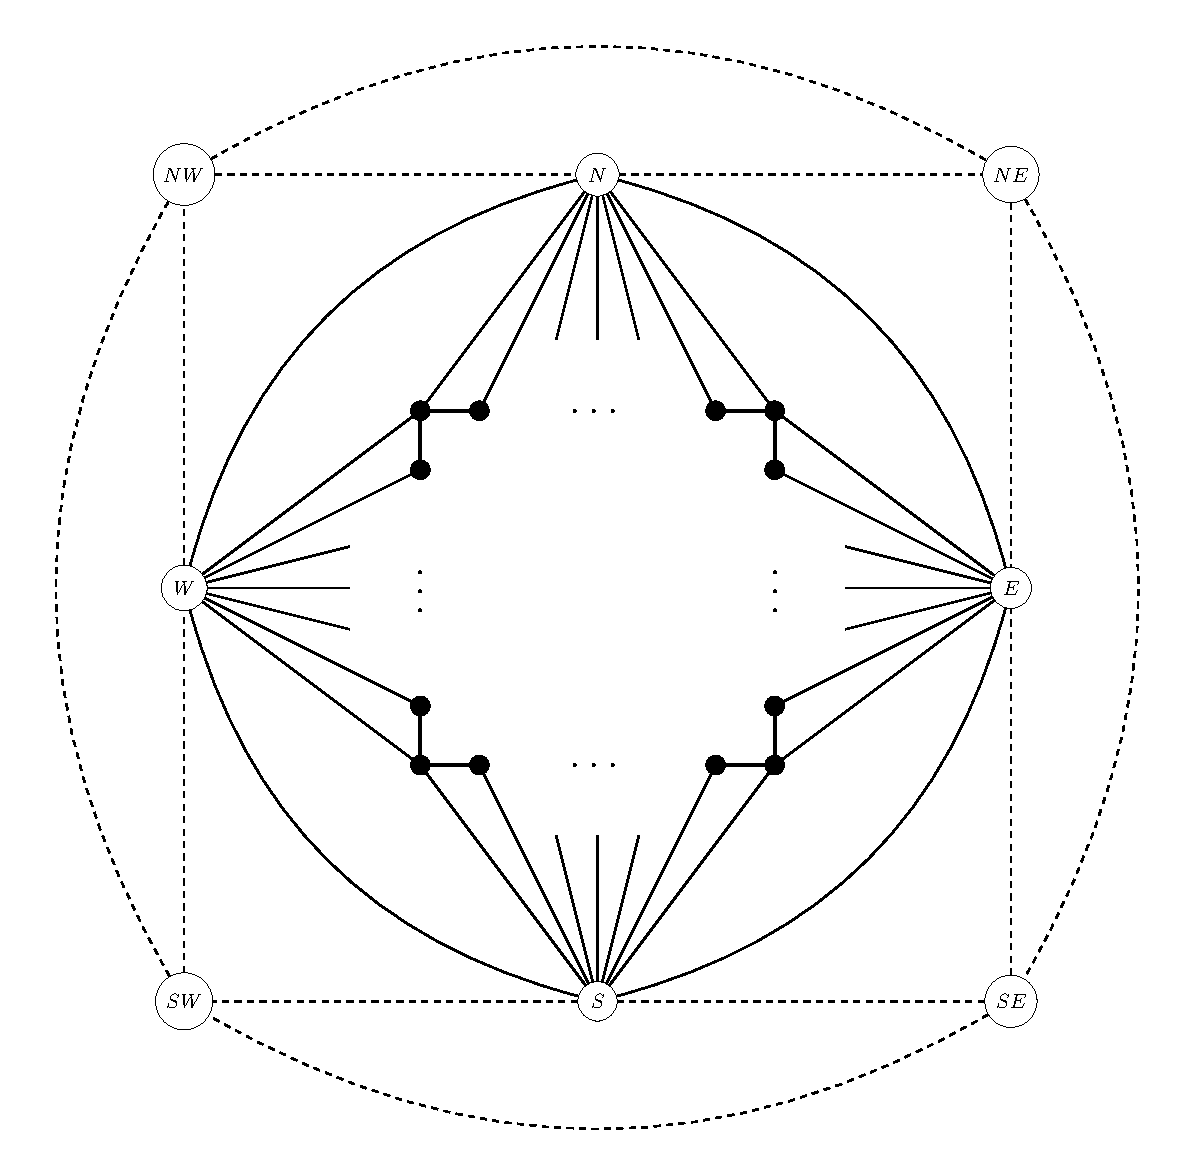
\includegraphics[scale=0.5]{fixExtension/img/scafold}

  \caption{The construction of a scaffold.
      \label{fig:scafold}}
  \end{figure}


  The graph $H$ can have more then one corner assignment but they all contain the separating $4$-cycle $\C= NESW$. Thus by Lemma \ref{lm:fix:fourCycleInteriorColor} we see that, without loss of generality, the interior edges of $\C$ incident to $N$ are colored incoming red, those incident to $E$ are colored incoming blue, those incident to $s$ are colored outgoing red and those incident to $W$ are colored outgoing blue.

\begin{proof}[Proof of Theorem \ref{fix:th:family}]
  Now all the preparations are done we can consider the family of graphs $G_k$ with the corner assignment $\ext G_k$ given in Figure \ref{fig:fix:manymany0}. We know we only have to look at this single corner assignment since we can force it with a scaffold. In $G_1$ the dots are replaced by a single vertex, in $G_2$ the dots are replaced by two vertices and so on. Each member has 2 maximal separating $4$-cycles. These are both marked by thick lines in Figure \ref{fig:fix:manymany0}.
  Many of the edges in this graph have only one possible color and orientation that does not violate the constraints of a regular edge labeling. Firstly, we can color the edges incident with the poles in accordance with the exterior vertex condition. Subsequently, we can use Lemma \ref{lm:fix:fourCycleInteriorColor} on both maximal separating $4$-cyles in accordance to color even more edges and finally we can color the edges in triangles of which the other two edges have  the same color using Lemma \ref{lm:rel:noMonoColoredTriangles}. These forced colorings are performed in Figure \ref{fig:fix:coloring}.

  \begin{figure}[h]
    \centering
    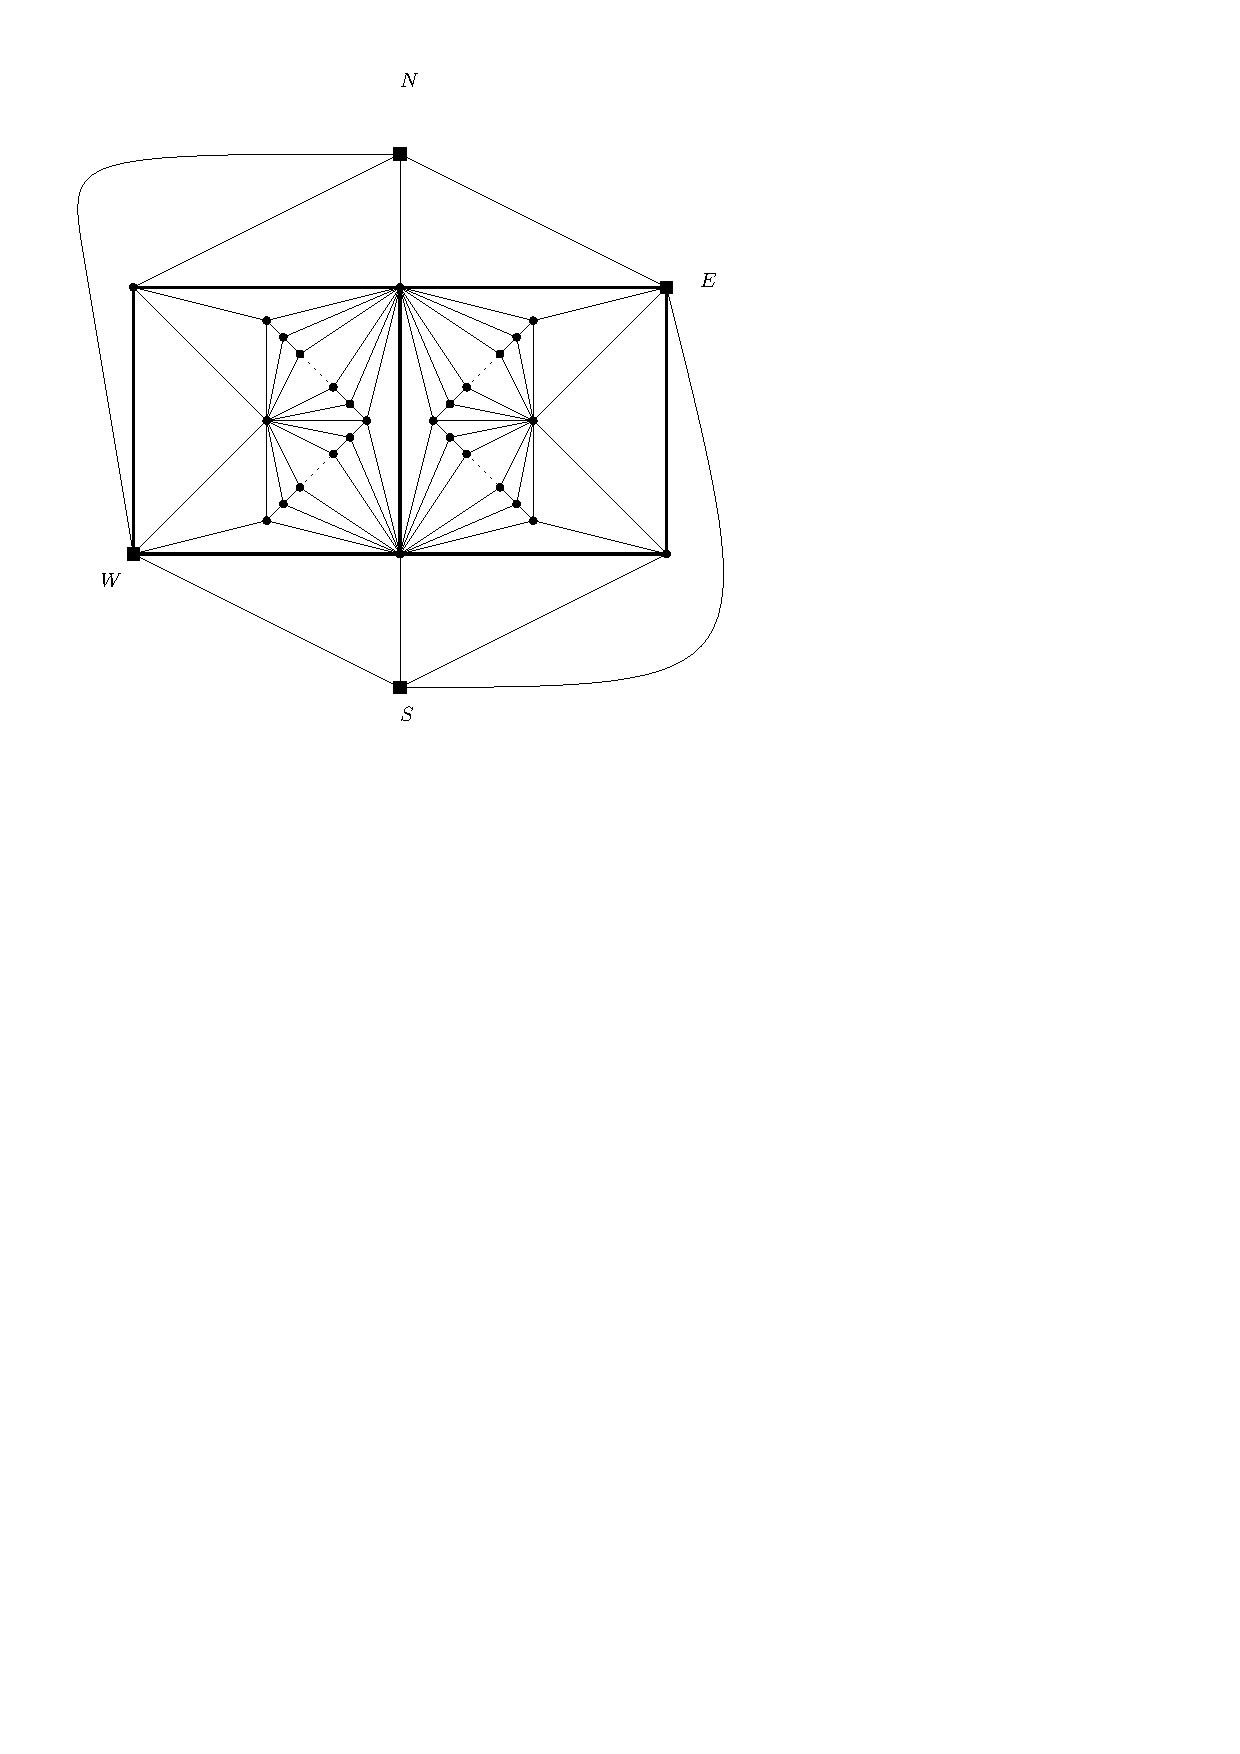
\includegraphics[scale=1]{fixExtension/img/manymanybase}
    \caption{A family of graphs not $k$-sided for any $k$}
    \label{fig:fix:manymany0}
  \end{figure}




  \begin{figure}[h]
    \centering
    \begin{subfigure}[t]{0.3\textwidth}
      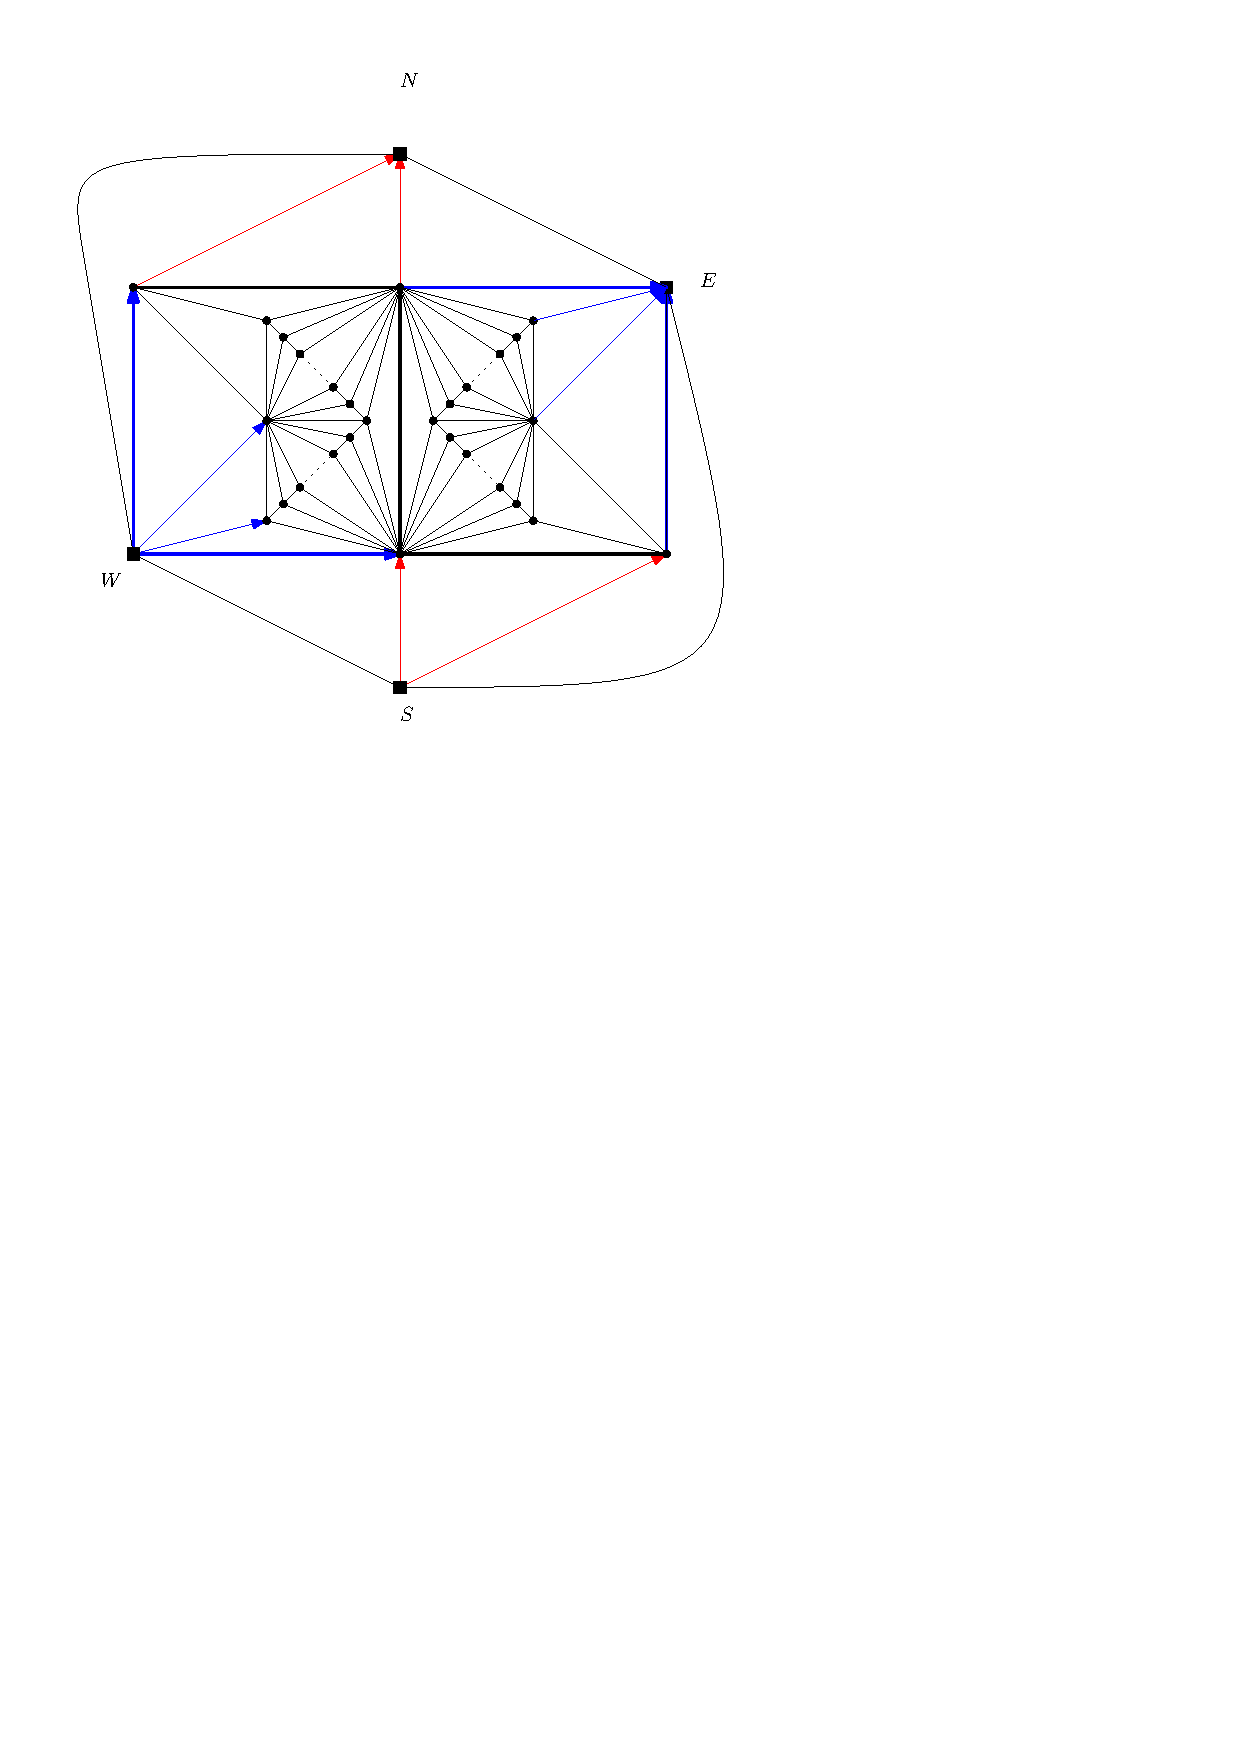
\includegraphics[width=\textwidth]{fixExtension/img/manymany1}
      \caption{Coloring the edges adjacent to the poles.}
      \label{fig:fix:manymany1}
    \end{subfigure}
    \quad
    \begin{subfigure}[t]{0.3\textwidth}
      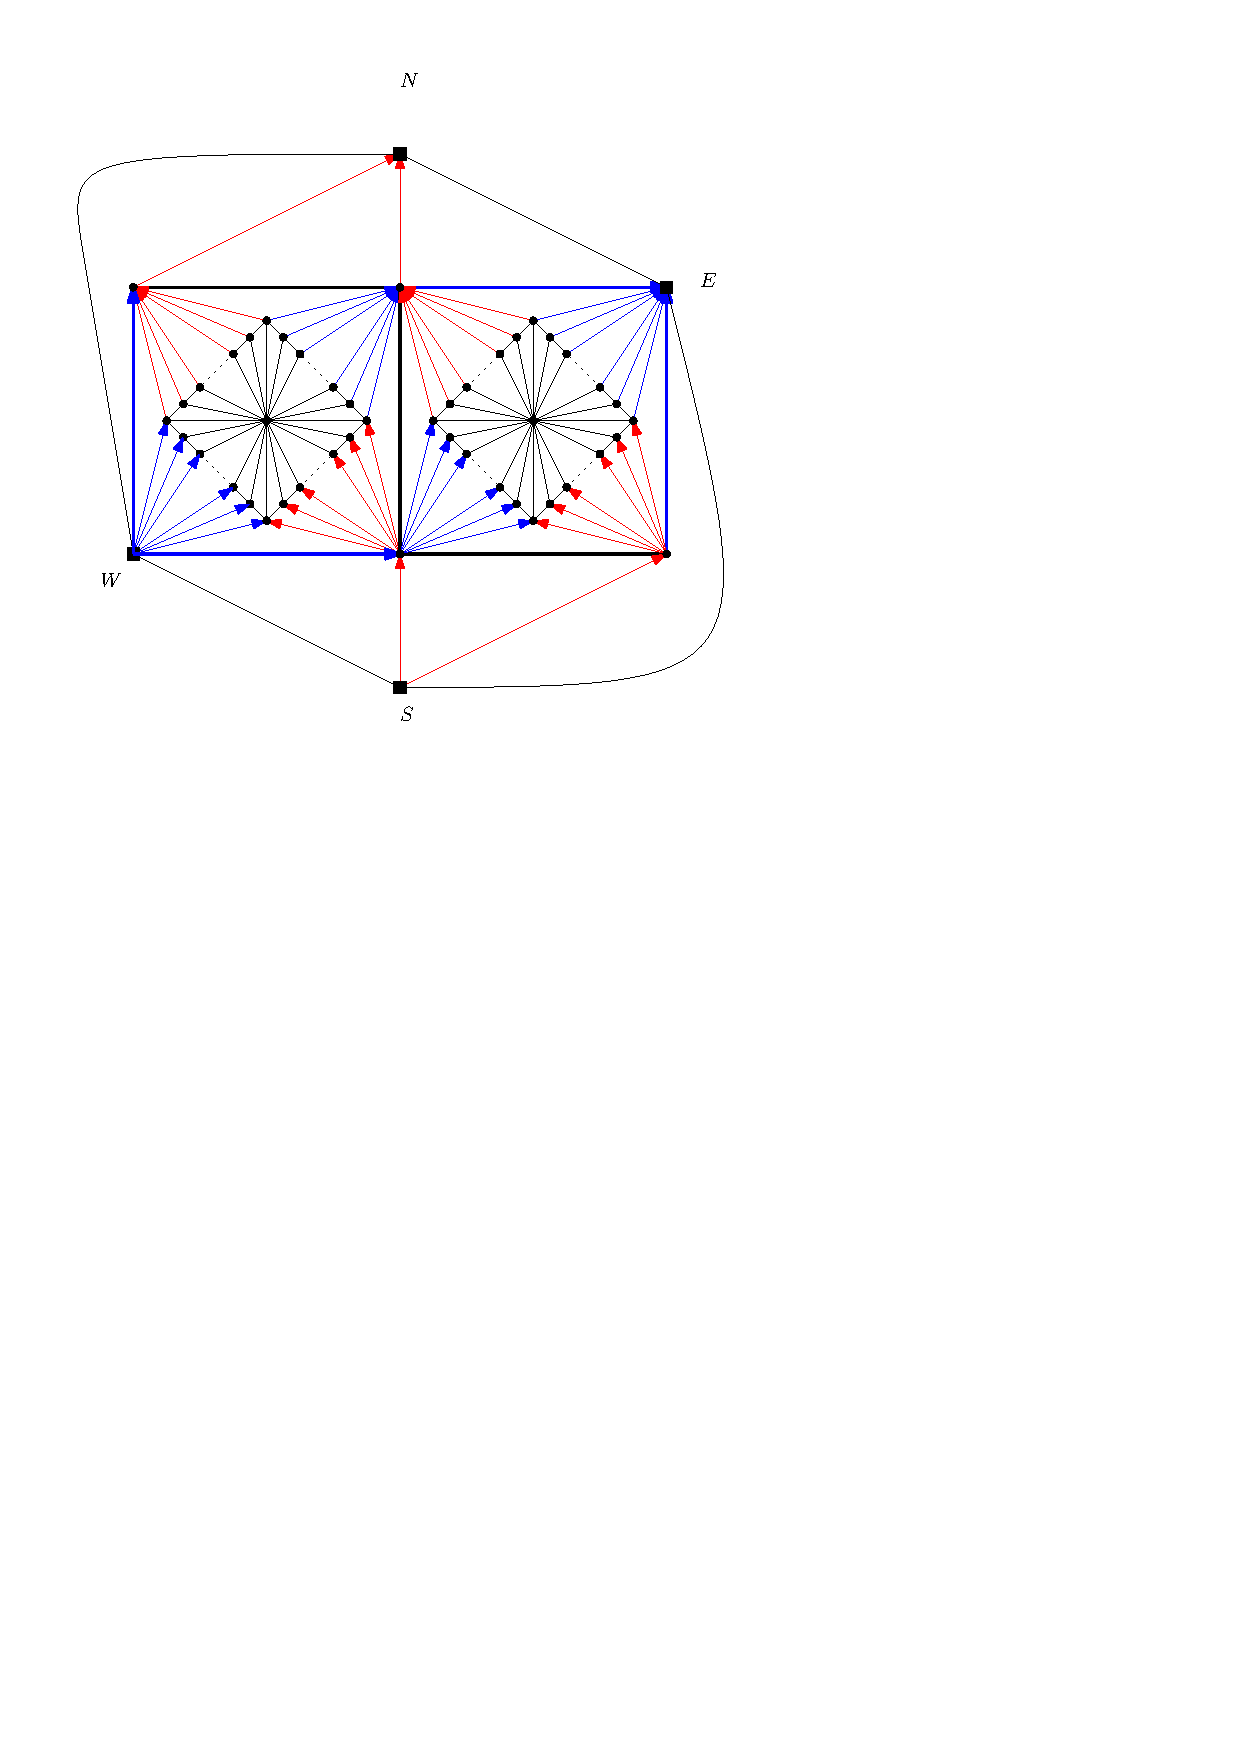
\includegraphics[width=\textwidth]{fixExtension/img/manymany2}
      \caption{Propagate trough the $4$-cycle.}
      \label{fig:fix:manymany2}
    \end{subfigure}
    \quad
    \begin{subfigure}[t]{0.3\textwidth}
      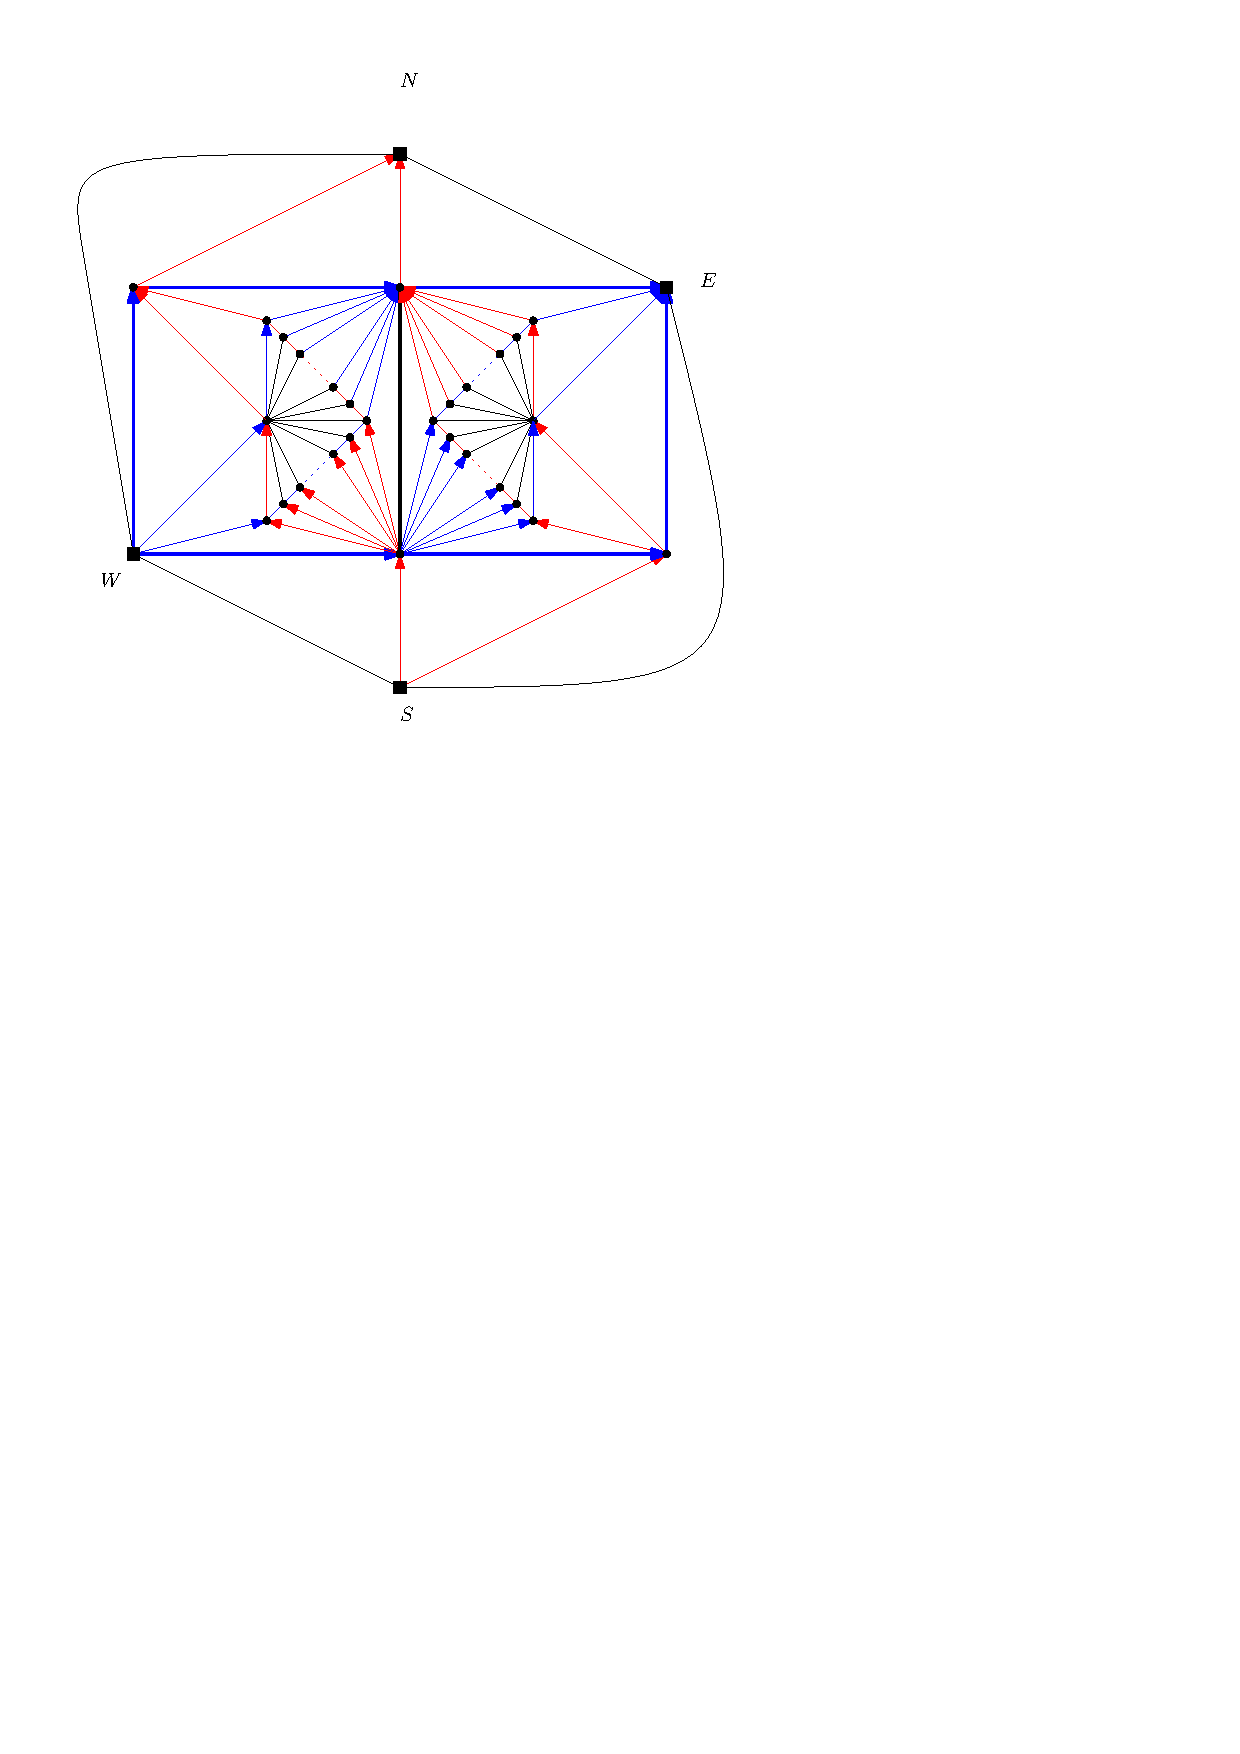
\includegraphics[width=\textwidth]{fixExtension/img/manymany3}
      \caption{Color such that there are no monochromatic triangles.}
      \label{fig:fix:manymany3}
    \end{subfigure}
    \caption{Coloring the graph.}
    \label{fig:fix:coloring}
  \end{figure}

  The result is then the graph displayed in Figure \ref{fig:fix:manymany4}. The black edges in this figure are edges that do not have a forced coloring by the above argument\footnote{Altough most of them can be forced by Lemma \ref{lm:fix:fourCycleInteriorColor}.}.
  We will focus on the centered black edge $e$, $e$ is an interior edges of both the red and blue faces that are drawn \fxnote*{change to dashed}{thick} in Figure \ref{fig:fix:manymany4}. These faces both have that both their boundary paths are of length larger then $k$ for a member $G_k$. Hence $e$ has to be colored both red and blue to prevent that face corresponding to a $k$-sided segment occurs in the final regular edge labeling. An edge can not be colored red and blue at the same time and hence $G_k$ is not $k$-sided.

  Since this proof doesn't depend on the value of $k$, the family $G_k$ has graphs that are not $k$-sided for any $k$.
\end{proof}


  \begin{figure}[h]
    \centering
    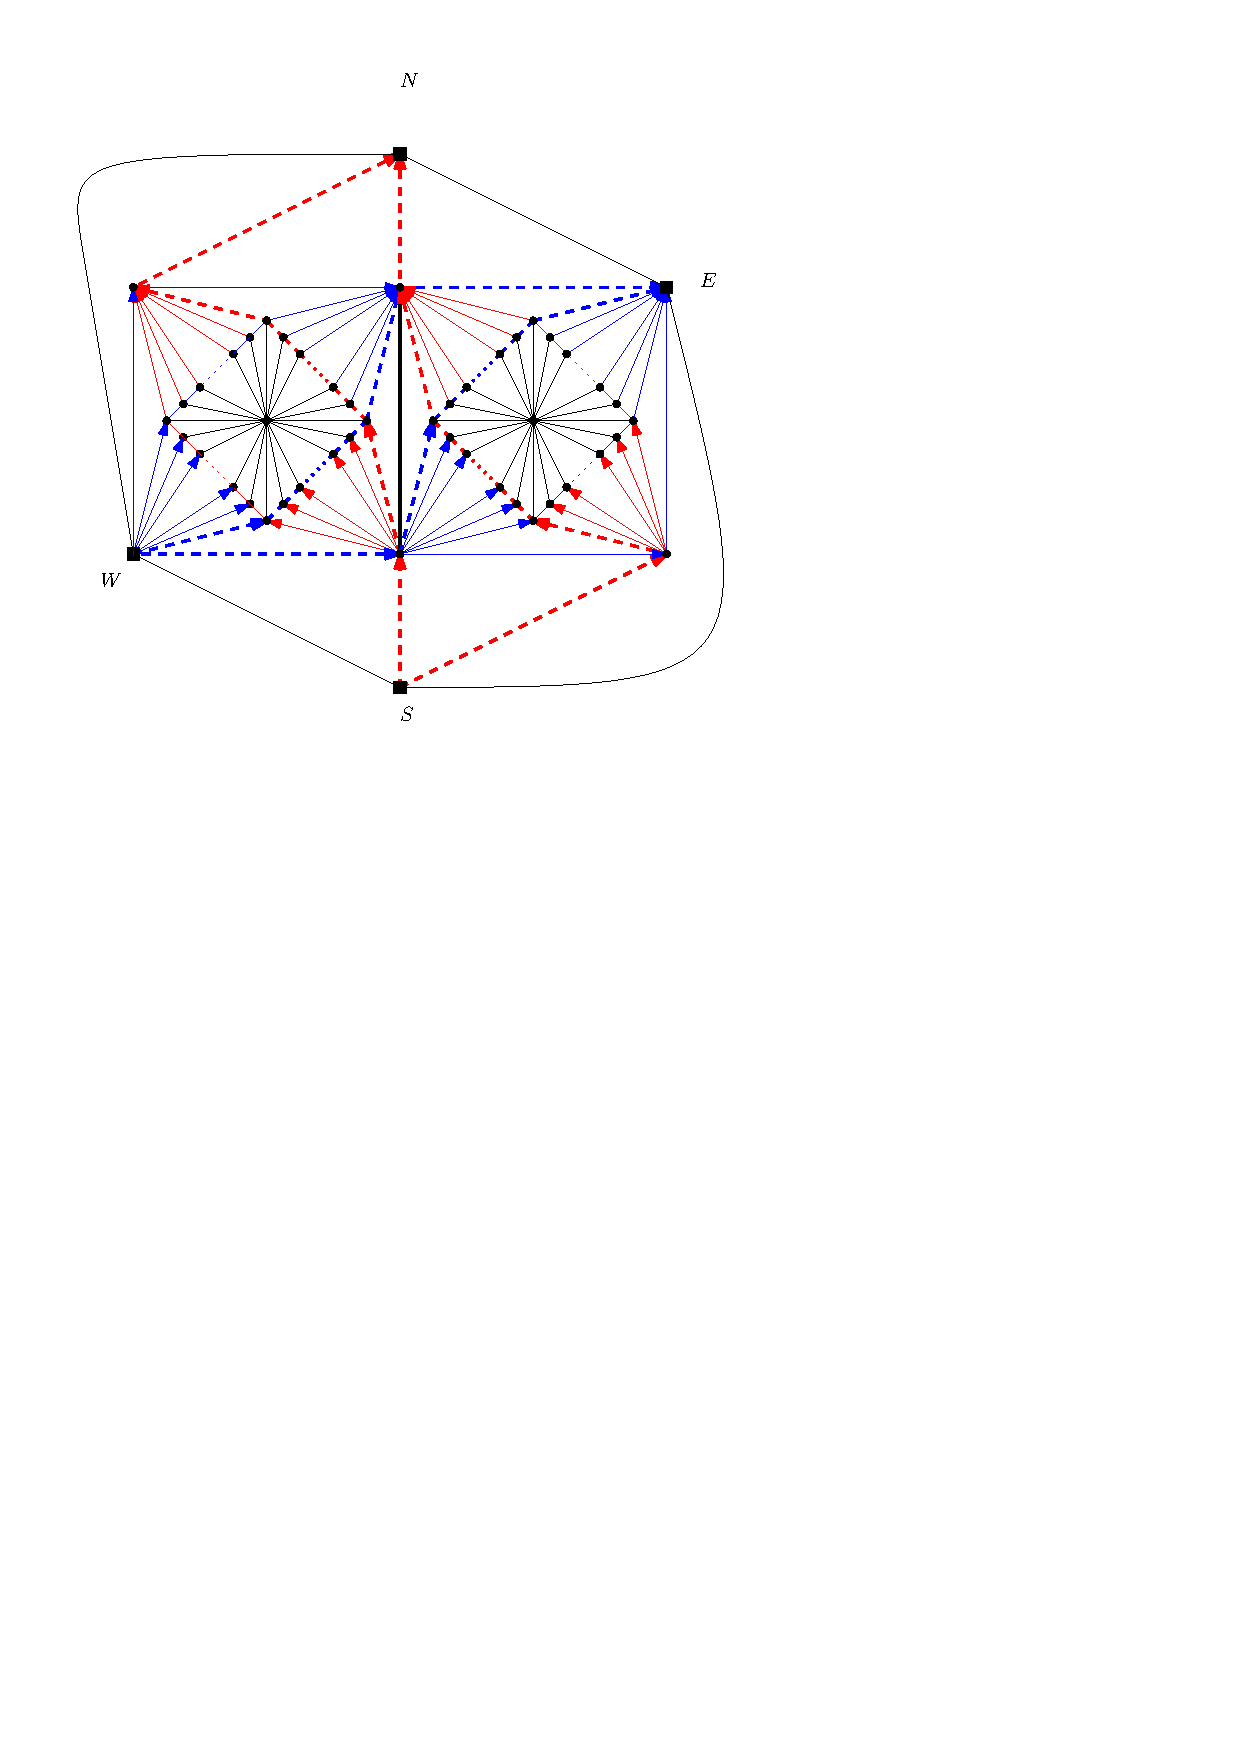
\includegraphics[scale=1]{fixExtension/img/manymany4}
    \caption{The graph after all coloring steps}
    \label{fig:fix:manymany4}
  \end{figure}
